\documentclass{beamer}
\usepackage[british]{babel}
\usepackage{times}
\usepackage{amsmath}
\usepackage{mathtools}
\usepackage{amsfonts}
\usepackage{verbatim}
\usepackage{lmodern}
\usepackage{tikz}
%\usepackage{algorithm}
\usetikzlibrary{patterns}


\DeclareMathOperator*{\argmax}{arg\,max}
\DeclareMathOperator*{\argmin}{arg\,min}

\DeclareMathOperator*{\KL}{{\rm KL}}

\begin{document}
\title{Master Project:\\Statistical analysis on genomic data}
\subtitle{Mid-term presentation}
\author{William van Rooij}
\institute{EPFL}
\date{12.04.19}
\logo{\includegraphics[width=30px]{images/EPFL_Logo.png}}
\maketitle
\begin{frame}
\begin{itemize}
\item Introduction
\item Variational inference
\item Mean-field approximation
\item Implementation
\item Results
\item Next steps
\end{itemize}
\end{frame}
\begin{frame}
\frametitle{Introduction}
\begin{itemize}
\item We introduce $X = (X_1,\ldots,X_p)$, and $y = (y_1,\ldots,y_q)$.
\item A SNP $X_s$ and a trait $y_t$, SNPs are strongly correlated.
\item Estimate the association between SNP $s$ and trait $t$.
\item $y_{n\times q} = x_{n\times p}\beta_{p \times q} + \epsilon_{n\times q}\text{, }\epsilon_t \sim \mathcal{N}(0,\tau_t^{-1}I_n)$
\item $y$ is a response matrix, $x$ are candidate predictors.

\item Each response $y_t$ is linearly related with the predictors and has a residual precision $\tau_t \sim $ Gamma$(\eta_t, \kappa_t)$.

\end{itemize}
\end{frame}
\begin{frame}
\frametitle{Introduction II}
\begin{itemize}
\item $s = 1,\ldots,p$, $t=1,\ldots,q$,
\item $\beta_{st}\mid\gamma_{st},\sigma^2,\tau_t \sim \gamma_{st}\mathcal{N}(0,\sigma^2\tau_t^{-1})+(1-\gamma_{st})\delta_0$,

(spike and slab)

\item $\gamma_{st} \mid \omega_{s} \sim $ Bernoulli$(\omega_s)$,

\item $\omega_s \sim $ Beta$(a_s,b_s)$,
\item $\tau_t \sim $ Gamma$(\eta_t,\kappa_t)$, $\sigma^{-2} \sim $ Gamma$(\lambda,\nu)$,
\item $a_s, b_s$ chosen to enforce sparsity. We define $p^*$ the expected number of predictors involved in the model, \textit{e.g.}:
$$
a_s \equiv 1\text{, }b_s \equiv q(p-p^*)/p^*
$$

\end{itemize}

\end{frame}

\begin{frame}
\frametitle{Introduction III}
\begin{itemize}
\item Markov Chain Monte Carlo algorithms (MCMC) are the usual way to approximate inference in relatively small datasets.
\item $p$ and $q$ are large compared to $n$.
\item MCMC gets time consuming, computational cost of operations increases with the number of parameters.
\item Number of iterations needed increases with the number of parameters.
\item Variational inference is an alternative to MCMC. 
\end{itemize}
\end{frame}

\begin{frame}
\frametitle{Variational inference}
\begin{itemize}
\item Observed data $\boldsymbol{y}$, parameters $\boldsymbol{\theta}$, posterior distribution of parameters $p(\boldsymbol{\theta} \mid \boldsymbol{y})$.
\item Approximate the posterior density with a simpler density $q$, minimizing a "closeness" measure: the Kullback-Leibler divergence.
\item $\KL(q\parallel p) := \int q(\boldsymbol{\theta})\log \left(\dfrac{q(\boldsymbol{\theta})}{p(\boldsymbol{\theta} \mid \boldsymbol{y})}\right) \mathrm{d}\boldsymbol{\theta}$.
\item Evidence lower bound (ELBO): $\mathcal{L}(q) = \mathbb{E}_q\left[\log p(\boldsymbol{\theta},\boldsymbol{y})\right] - \mathbb{E}_q\left[\log q(\boldsymbol{\theta})\right]$.
\item $\KL(q\parallel p) = \log(p) - \mathcal{L}(q)$.
\item Minimizing KL is equivalent to maximizing ELBO.
\end{itemize}
\end{frame}

\begin{frame}
\frametitle{Mean-field approximation}
\begin{itemize}
\item We assume independence for most of the parameters:
$$
q(\boldsymbol{\theta}) = \left\lbrace\prod_{s=1}^p\prod_{t=1}^qq(\beta_{st},\gamma_{st})\right\rbrace\left\lbrace\prod_{s=1}^pq(\omega_s)\right\rbrace\left\lbrace\prod_{t=1}^qq(\tau_t)\right\rbrace q(\sigma^{-2}).
$$
\item The mean-field approximation does not represent the correlations between parameters.
\end{itemize}
\begin{figure}
\centering
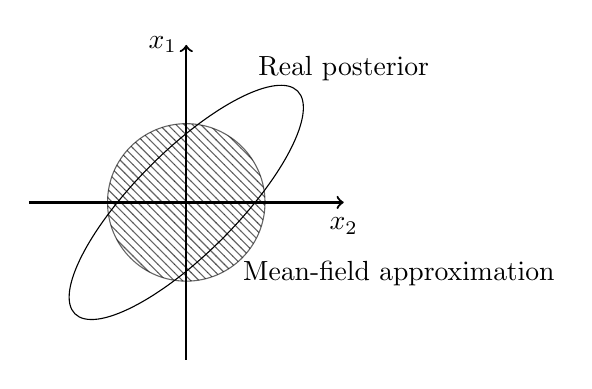
\begin{tikzpicture}
\draw[thick, ->] (0,-2) -- (0,2);
\draw[thick, ->] (-2,0) -- (2,0);
\fill[pattern=north west lines,opacity=.6,draw] (0,0) circle (1cm);
\draw[rotate=-45] (0,0) ellipse (0.65cm and 2cm);
\node (p) at (2,1.7) {Real posterior};
\node (q) at (2.7,-0.9) {Mean-field approximation};
\node (x1) at (-0.3,2) {$x_1$};
\node (x2) at (2,-0.3) {$x_2$};
\end{tikzpicture}\end{figure}
\end{frame}

\begin{frame}
\frametitle{Coordinate ascent variational inference - CAVI}
\begin{itemize}
\item If we fix $q_l(\theta_l)$, $l \neq j$, the optimal for $q_j(\theta_j)$ verifies: $q^*_j(\theta_j) \propto \exp\left\lbrace\mathbb{E}_{-j}\left[\log p(\theta_j \mid \boldsymbol{\theta}_{-j},\boldsymbol{y}\right]\right\rbrace$
\item \begin{text}
IN: $p(x,z)$, data set $x$, tolerance $tol$,\\
OUT: $q(z) = \prod q_j(z_j)$.\\
INIT: $q_j(z_j)$, \\
REPEAT:\\
\quad FOR: $j \in \left\lbrace1, \dots, m\right\rbrace$,\\
\quad \quad SET: $q_j(z_j) \propto \exp\left\lbrace\mathbb{E}_{-j}\left[\log p(z_j|z_{-j},x)\right]\right\rbrace$.\\
\quad COMPUTE:\\
\quad \quad $ELBO^{old}(q) \leftarrow ELBO(q)$.\\
\quad \quad $ELBO(q) = \mathbb{E}\left[\log p(z,x)\right] - \mathbb{E}\left[\log q(z) \right] $.\\
UNTIL: $|ELBO(q)-ELBO^{old}(q)|<tol$.\\
RETURN: $q(z).$
\end{text}
\end{itemize}
\end{frame}

\begin{frame}
\frametitle{Coordinate ascent variational inference - CAVI II}
\begin{itemize}
\item $\mathcal{L}(q)$ is guaranteed to increase at every iteration.
\item We assume there exists a best model and we want to find it
\item CAVI yields a local optimum, depending on the initialization of the parameters.
\item Another possible solution is annealing, which consists of "heating" the distribution to have only a global maximum.
\item Annealing yields a unique model, so averaging might better represent the incertitude.
\end{itemize}
\end{frame}

\begin{frame}
\frametitle{Parameters distributions}
\begin{itemize}
\item $\beta_{st} \mid \gamma_{st} = 1, \boldsymbol{y} \sim \mathcal{N}\left(\mu_{\beta,st},\sigma_{\beta,st}^2\right)$,
\item $\beta_{st} \mid \gamma_{st} = 0, \boldsymbol{y} \sim \delta_0$,
\item $\gamma_{st} \mid \boldsymbol{y} \sim $ Bernoulli$(\gamma_{st}^{(1)})$,
\item $\omega_s \mid \boldsymbol{y} \sim $ Beta$(a^*_s, b^*_s)$,
\item $\tau_t \mid \boldsymbol{y} \sim $ Gamma$(\eta_t^*, \kappa_t^*)$,
\item $\sigma^{-2} \mid \boldsymbol{y} \sim $ Gamma$(\lambda^*,\nu^*)$,
\end{itemize}
\end{frame}

\begin{frame}
\frametitle{"Bayesian model averaging"}
\begin{itemize}
\item Denote $M_k$, $k= 1,\ldots, K$ the models yielded by the local optimums.
\item $p(\gamma_{st} \mid \boldsymbol{y}) = \sum_{k=1}^{K}p(\gamma_{st}\mid M_k)p(M_k \mid \boldsymbol{y})$,
\item $p(M_k \mid \boldsymbol{y}) = \dfrac{p(\boldsymbol{y} \mid M_k)p(M_k)}{\sum_{j=1}^{K}p(\boldsymbol{y}\mid M_j)p(M_j)},$
\item $\mathcal{L}(q)$ serves as an approximation of $\log p(\boldsymbol{y} \mid M_k)$, as $\KL(q\parallel p) = \log p(\boldsymbol{y}) - \mathcal{L}(q)$.
\item $p(M_k)$ is the prior probability of the models, we consider them to be equiprobable: $p(M_k) = 1/K$, $\forall k = 1,\ldots,K$.
\end{itemize}
\end{frame}

\begin{frame}
\frametitle{Implementation}
\begin{itemize}
\item Generate SNPs, traits, and associations.
\item Find the optimums $q^*(\boldsymbol{\theta})$ with different initial parameters, drawn at random.
\item Generate the ELBOs and use them as weights in the weighted average ("BMA").
\item The function yields probabilities of association between SNPs and traits.
\end{itemize}
\end{frame}




\begin{frame}
\frametitle{Results}
\begin{itemize}
\item $n = 300$ observations,
\item $p = 500$ SNPs, with $p_0$ associated SNPs,
\item $q = 1$ trait, %for visualisation
\item $100$ random initialisations,
\item autocorrelation between the SNPs is between $0.95$ and $0.99$, in blocks of ten SNPs,
\item we can specify the maximum proportion of response variance explained by the SNPs.
\item We used $50$ replications to determine the ROC curves.
\end{itemize}
\end{frame}



\begin{frame}
\frametitle{Weighted averaging with $p_0 = 5$, max var. $=0.5$}
\begin{figure}
\includegraphics[width=2.1in]{images/CorrSingle.png}
\includegraphics[width=2.1in]{images/CorrWeights.png}
\end{figure}
\end{frame}


\begin{frame}
\frametitle{ROC curves comparison, $p_0 = 15$, max var.$=0.5$}
\begin{figure}
\includegraphics[width=3in]{images/ROC_Comp_p0_15_var_0_5.jpeg}
\end{figure}
\end{frame}
\begin{frame}
\frametitle{ROC curves comparison, $p_0 = 15$, max var.$=0.8$}
\begin{figure}
\includegraphics[width=3in]{images/ROC_Comp_p0_15_var_0_8.jpeg}
\end{figure}
\end{frame}
\begin{frame}
\frametitle{ROC curves comparison, $p_0 = 50$, max var.$=0.5$}
\begin{figure}
\includegraphics[width=3in]{images/ROC_Comp_p0_50_var_0_5.jpeg}
\end{figure}
\end{frame}
\begin{frame}
\frametitle{ROC curves comparison, $p_0 = 50$, max var.$=0.8$}
\begin{figure}
\includegraphics[width=3in]{images/ROC_Comp_p0_50_var_0_8.jpeg}
\end{figure}
\end{frame}

\begin{frame}
\frametitle{Results}
\begin{itemize}
\item Paralleled computation is possible.
\item The difference is bigger when phenotypic variance is better explained from the SNPs.
\item The difference is bigger with fewer active SNPs.
\end{itemize}
\end{frame}

\begin{frame}
\frametitle{Next steps}
\begin{itemize}
\item Optimization of the code, $\rightarrow$ ev. integration to R-package,
\item Comparison with annealing and non-weighted averaging for strong correlations.
\item Do we find the right modes? 2D visualisations (Rocková).
\item Application to real data.

\end{itemize}
\end{frame}

\begin{frame}
Thank you for your time.
\end{frame}
\end{document}